\chapter{Introduction}\label{chap:intro}

A main class of multi-agent assignment problems is \emph{cooperative coordination}, which
considers the synergies between agents that have common goals \cite{shoham2008mas}. In
multi-robot systems, it is called \emph{Multi-Robot Task Allocation} (MRTA)
\cite{gerkey2004}. Within this class, we are interested in problems involving both routing
and scheduling, which are crucial in areas of increasing importance such as precision
agriculture, environmental monitoring, warehouse automation, pickup and delivery,
last-mile planning, space exploration, and disaster response \cite{nunes2017taxonomy}.

In this thesis, we study large-scale, dynamic and distributed cooperative coordination,
with focus on disaster response scenarios \cite{rcr2001,murphy2014}. We explain the
challenges of disaster response in Section \ref{sec:domain}, and state our problem in
Section \ref{sec:pstat}. We summarise our research objectives and methodology in Section
\ref{sec:objectives}. Finally, we highlight our contributions in Section
\ref{sec:contrib}, and outline the structure of the document in Section \ref{sec:outline}.

\section{Motivating Domain: Disaster Response}\label{sec:domain}

The information age is plagued by all kinds of disasters. Through the screens of our
smart devices, we helplessly witness events such as wildfires, explosions, earthquakes,
and volcanic eruptions. Although there is no generally accepted terminology, modern
disaster management can be divided into the following phases
\cite{alexander2002,hawe2012survey}:
\begin{enumerate}
    \item \emph{Mitigation}: reducing or eliminating the possibility of a disaster;
    \item \emph{Preparation}: equipping humans with the means to increase their survival
        and to minimise the losses during a disaster;
    \item \emph{Response}: reducing or eliminating the impact of a disaster;
    \item \emph{Recovery}: restoring the situation to the state prior to the impact of a
        disaster.
\end{enumerate}
\begin{figure}[t]
    \centering
    \begin{adjustbox}{width=.4\textwidth}
        \begin{tikzpicture}
    \tiny

    \draw[-{Implies},double,line width=0.25] (-1,  0) to [bend left=45] ( 0,  1);
    \draw[-{Implies},double,line width=0.25] ( 0,  1) to [bend left=45] ( 1,  0);
    \draw[-{Implies},double,line width=0.25] ( 1,  0) to [bend left=45] ( 0, -1);
    \draw[-{Implies},double,line width=0.25] ( 0, -1) to [bend left=45] (-1,  0);

    \node[fill=white,inner sep=0,outer sep=0] at (-0.75, 0.5) {Mitigation};
    \node[fill=white,inner sep=0,outer sep=0] at (0.75, 0.5) {Preparation};
    \node[fill=white,inner sep=0,outer sep=0] at (0.75, -0.5) {Response};
    \node[fill=white,inner sep=0,outer sep=0] at (-0.75, -0.5) {Recovery};
\end{tikzpicture}

    \end{adjustbox}
    \caption[The disaster management cycle]{The disaster management cycle
        \cite{alexander2002}. The mitigation and preparation phases try to prevent
        disasters with measures such as keeping evacuation plans up to date and minimising
        safety issues. The response phase focuses mainly on saving and safeguarding human
        lives, while the recovery phase is dedicated to repair damage, which in some cases
        can take years.}
    \label{fig:dr}
\end{figure}
Regardless of how effective the mitigation and preparation phases may be, they are unable
to eliminate every possible hazard \cite{coppola2006}. Thus, the response phase plays an
important role in the disaster management cycle. It consists of a set of complex actions
like search and rescue, first aid and infrastructure restoration, which are carried out
during periods of high stress, in severely time-constrained environments, and with limited
information. In this phase, it is fundamental to plan firmly and act as fast as possible,
since any delay can lead to further tragedy and destruction.

Consider the aftermath of a disaster, either natural, like the Cumbre Vieja volcanic
eruption in 2021, or man-made, like the Beirut explosion in 2020. Different actors can be
present, such as first responders, aid organisations, news reporters and local citizens.
The first objective is to assess the situation and determine what are the problems to
solve. For this purpose, UAVs may be deployed to patrol the affected areas, sensors may be
used to monitor the environment, and citizens may contribute using social media platforms
such as Ushahidi \cite{ushahidi} or Google Crisis Response. From heterogeneous sources, a
great variety of content will be generated, such as maps, forecasts and reports. Once a
set of tasks has been identified, a set of agents will be defined to perform them, each
with its specific resources and capabilities. Then, the response phase will take place in
the following steps \cite{hac2014}:
\begin{enumerate}
    \item \emph{Formation}: agents jointly define how tasks are allocated. To encourage
        commitment, incentive schemes could be put in place (e.g., completing
        high-priority tasks could be paid double);
    \item \emph{Operation}: agents perform the tasks allocated to them. The execution is
        not straightforward: more critical tasks may appear, new agents or resources may
        become available, or current agents may disengage (e.g., a UAV could fall due to a
        malfunction and be destroyed). Therefore, agents must monitor the system status
        continuously, and redefine assignments if necessary;
    \item \emph{Disbandment}: the collective is disbanded either when all tasks have been
        successfully completed, or the emergence of some condition prevents continuation
        (e.g., a sudden fire spread impedes access to an area of interest, and no
        firefighters are available at the moment). After that, any rewards, such as
        payments, transfer of privileges or additional information, are distributed among
        agents.
\end{enumerate}

\begin{figure}[t]
    \centering
    \begin{subfigure}[b]{.325\textwidth}
        \includegraphics[width=\textwidth]{example1}
    \end{subfigure}
    \begin{subfigure}[b]{.325\textwidth}
        \includegraphics[width=\textwidth]{example2}
    \end{subfigure}
    \begin{subfigure}[b]{.325\textwidth}
        \includegraphics[width=\textwidth]{example3}
    \end{subfigure}
    \caption[Examples of cooperative coordination in disaster response]{%
    Examples of cooperative coordination in disaster response. From left to right: USV
    inspecting piers after Hurricane Wilma \cite{murphy2014}; the Colossus robot assisting
    the Paris Fire Brigade in the fight against the $2019$ Notre Dame Cathedral fire
    \cite{colossus}; fire-fighting UAVs in the Dazu District, China \cite{dazu}.}
\end{figure}

\iffalse
Oother motivating domains:
   - resource allocation (e.g., hospital workforce)
   - vehicle routing
   - combine harvesting
   - multi-factory scheduling
   - project scheduling
   - automated guided vehicles
   - open vehicle fleets
   - green maritime transportation
   - sensor networks
\fi

As can be seen, disaster response provides a comprehensive example of the various
challenges of cooperative coordination. In fact, it is a central class of case studies for
the multi-agent/robot systems community
\cite{rcr2001,murphy2014,dadvar2021,murphy2016a,murphy2016b}, as well as for AI in general
\cite{imran2014}. Based on this domain, we identify our problem below.

\section{Problem Statement}\label{sec:pstat}

We focus on the \emph{Coalition Formation with Spatial and Temporal constraints Problem}
(CFSTP) \cite{ramchurn2010cfstp}. We use the definitions of \emph{coalition} and
\emph{coalition formation} given by \cite{horling2005}. Hence, a coalition is a flat and
task-oriented organisation of agents, short-lived and disbanded when no longer needed,
while coalition formation is a consequence of the emergent behaviour of the system
\cite{mataric1993}.
Regardless of its current location, an agent is considered part of a coalition from the
moment it is assigned a task, to the moment the task is completed.
We consider coalitions to be different from teams (Figure \ref{fig:coalition-team}).
Moreover, based on \cite[Section $4.5$]{nunes2017taxonomy}, we consider a system to be
\emph{real-time} if it may have \emph{hard} deadlines, which cannot be violated, and
possibly also \emph{soft} deadlines, which can be violated with some penalty.
In the CFSTP, tasks (e.g., save victims or put out fires) have to be assigned to agents
(e.g., ambulances or fire brigades). The assignment is determined by the spatial
distribution of tasks in the disaster area, the time needed to reach them, the
workload they require (e.g., how large a fire is) and their deadlines (e.g., estimated
time left before victims perish). In addition to these constraints,
the number of agents may be much smaller than the number of tasks, hence they need to
cooperate with each other by forming, disbanding and reforming coalitions over time
\cite{shehory1998,epstein2011}.
The objective of the CFSTP is to define which tasks (e.g., sites with the most victims and
the strongest fires) to allocate to which coalitions (e.g., the fastest ambulances and
fire engines with the largest water tanks), in order to maximise the number of tasks
completed.
\begin{figure}[t]
    \centering
    \begin{subfigure}[b]{.49\textwidth}
        \centering
        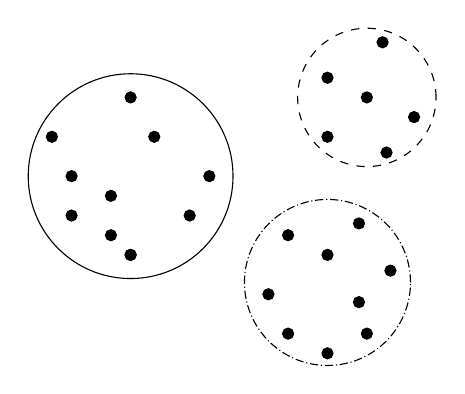
\begin{tikzpicture}
    \node at (-0.25, 0.25) {\pgfuseplotmark{*}};
    \node at (-0.75, 0.5 ) {\pgfuseplotmark{*}};
    \node at (0.75 , 0.5 ) {\pgfuseplotmark{*}};
    \node at (0    , 0   ) {\pgfuseplotmark{*}};
    \node at (1    , 1   ) {\pgfuseplotmark{*}};
    \node at (-0.75, 1   ) {\pgfuseplotmark{*}};
    \node at (-1   , 1.5 ) {\pgfuseplotmark{*}};
    \node at (-0.25, 0.75) {\pgfuseplotmark{*}};
    \node at (0    , 2   ) {\pgfuseplotmark{*}};
    \node at (0.3  , 1.5 ) {\pgfuseplotmark{*}};
    \node at (0    , 0   ) {\pgfuseplotmark{*}};

    \draw (0, 1) circle (37pt);

    \node at (2.5 , -1.25) {\pgfuseplotmark{*}};
    \node at (2   , -1   ) {\pgfuseplotmark{*}};
    \node at (3   , -1   ) {\pgfuseplotmark{*}};
    \node at (1.75, -0.5 ) {\pgfuseplotmark{*}};
    \node at (2.5 ,  0   ) {\pgfuseplotmark{*}};
    \node at (2   ,  0.25) {\pgfuseplotmark{*}};
    \node at (2.9 , -0.6 ) {\pgfuseplotmark{*}};
    \node at (2.9 ,  0.4 ) {\pgfuseplotmark{*}};
    \node at (3.3 , -0.2 ) {\pgfuseplotmark{*}};

    \draw[densely dashdotted] (2.5, -0.35) circle (30pt);

    \node at (3   , 2    ) {\pgfuseplotmark{*}};
    \node at (3.2 , 2.7  ) {\pgfuseplotmark{*}};
    \node at (3.6 , 1.75 ) {\pgfuseplotmark{*}};
    \node at (2.5 , 1.5  ) {\pgfuseplotmark{*}};
    \node at (2.5 , 2.25 ) {\pgfuseplotmark{*}};
    \node at (3.25, 1.3  ) {\pgfuseplotmark{*}};

    \draw[dashed] (3, 2) circle (25pt);
\end{tikzpicture}

        \caption{Coalitions.}
    \end{subfigure}
    \hfill
    \begin{subfigure}[b]{.49\textwidth}
        \centering
        \raisebox{12pt}{
            \begin{adjustbox}{width=.9\textwidth}
                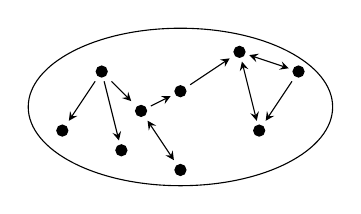
\begin{tikzpicture}
    \node (n1) at (0   , 0    ) {\pgfuseplotmark{*}};
    \node (n2) at (0.25, -1   ) {\pgfuseplotmark{*}};
    \node (n3) at (0.5 , -0.5 ) {\pgfuseplotmark{*}};
    \node (n4) at (-0.5, -0.75) {\pgfuseplotmark{*}};
    \node (n5) at (1   , -0.25) {\pgfuseplotmark{*}};
    \node (n6) at (1   , -1.25) {\pgfuseplotmark{*}};
    \node (n7) at (1.75, 0.25 ) {\pgfuseplotmark{*}};
    \node (n8) at (2.5 , 0    ) {\pgfuseplotmark{*}};
    \node (n9) at (2   , -0.75) {\pgfuseplotmark{*}};

    %\begin{scope}[-Straight Barb]
    \begin{scope}[-stealth]
    \draw (n1) -- (n2);
    \draw (n1) -- (n3);
    \draw (n1) -- (n4);
    \draw (n3) -- (n5);
    \draw (n5) -- (n7);
    \draw (n8) -- (n9);
    \end{scope}

    %\begin{scope}[Straight Barb-Straight Barb]
    \begin{scope}[stealth-stealth]
    \draw (n3) -- (n6);
    \draw (n7) -- (n8);
    \draw (n7) -- (n9);
    \end{scope}

    \draw (1, -0.45) ellipse (55pt and 1cm);
\end{tikzpicture}

            \end{adjustbox}}
        \caption{A team.}
    \end{subfigure}
    \caption[Differences between coalitions and teams]{%
        Differences between coalitions and teams \cite{horling2005}. Once formed, a
        coalition becomes an atomic entity that exists for a limited time, such
        as political parties joining together to form a government. In contrast, a team
        is a long-term organisation in which agents may have different roles, as in the
        game of football.}
    \label{fig:coalition-team}
\end{figure}

Despite having similarities with classic problems such as Generalised Assignment Problem
\cite{ross1975} and Job-Shop Problem \cite{brucker2007}, the importance of the CFSTP lies
in the fact that it was the first generalisation of the \emph{Team Orienteering Problem}
(TOP) to consider coalition formation \cite[Section $4.2$]{ramchurn2010cfstp}. For this
reason, it has been applied in contexts such as human-agent collectives
\cite{ramchurn2015a}, multi-UAV exploration \cite{baker2016}, and law enforcement
\cite{nelke2020,tkach2021}.

Within this problem class, our interest is in algorithms that are anytime (i.e., which can
return partial solutions if they are interrupted before completion), efficient, and have
theoretical properties. In other words, approximate algorithms \cite{papadimitriou1993}.
The reason is that they are fundamental in real-time domains, where it is necessary to
have provable guarantees, but it may be computationally not feasible or economically
undesirable to produce an optimal solution \cite{zilberstein1996,calvaresi2021}. In
particular, as we said above, the faster the disaster response, the lower the losses
incurred. We also assume that the agents are situated in a distributed system
\cite{tanenbaum2017} with a \emph{dynamic evolution of the environment}\footnote{Also
referred to as \emph{open} systems \cite{hewitt1990}. For brevity, we call them
\emph{dynamic environments}.} \cite{fioretto2018survey}, that is:
\begin{enumerate}
    \item It must be possible for agents to reach a solution through local interaction,
        rather than relying on a centralised solver \cite{ramchurn2010fms};
    \item At any time, agents can join in or leave, and new tasks can appear.
\end{enumerate}
If the problem is solved in a centralised fashion, then the designated solver has to be
informed whenever there is a change, recompute the solution, and redistribute it to all
agents.
In real-time domains such as disaster response, this leads to three major issues. First, a
centralised solver is a single point of failure that makes the system fragile and not
robust to unexpected events, such as malfunctions or communication disturbances between
agents far apart \cite{petcu2007thesis}. Second, if the agents have limited computational
resources and the problem is not small, electing a centralised solver might not be
possible, while distributing computations always improves scalability
\cite{tanenbaum2017}. Third, a centralised approach might not be as effective as a
distributed one, given that the situation can evolve rapidly and there could be
significant communication delays \cite{mailler2018}.

\section{Research Objectives and Methodology}\label{sec:objectives}

We aim to develop models, algorithms and test frameworks for multi-agent coordination,
with the following requirements.
\begin{description}[style=nextline]
    \item[R1] \emph{Decentralised autonomy}: the agents do not have to rely on a single
        point of failure. This is particularly important for disaster scenarios, where
        unreliable infrastructures and scarce supplies imply that lost resources cannot
        be replaced.
    \item[R2] \emph{Cooperation}: the agents have to coordinate their actions so to
        maximise their performance. Cooperation is also necessary when tasks require
        combined skills. For example, to extract survivors from the rubble of a collapsed
        building, rescue robots detect life signs with their sensors, firefighters dig and
        paramedics load the injured into ambulances.
        Therefore, the solutions must focus on achieving a global objective.
    \item[R3] \emph{Scalability}: the algorithms have to target scenarios with tens to
        thousands of agents and tasks, in order to be usable in future contexts where
        mass deployment of agents (e.g., robot swarms) will be common.
    \item[R4] \emph{Resilience}: agents and resources could be added and removed at any
        time, either by a human supervisor or due to unexpected failures. The algorithms
        must be able to produce feasible solutions even in such situations. If the
        solution quality degrades, it must happen in a controlled way.
\end{description}
Moreover, motivated by the disaster response domain, and intending to address the main
open issues in the MRTA literature \cite[Section $9.2$]{nunes2017taxonomy}, we make the
following assumptions.
\begin{description}[style=nextline]
    \item[A1] Tasks have spatio-temporal constraints (e.g., the buildings on fire are
        scattered throughout the city, and each will burn out completely after a certain
        amount of time). In particular, each task has a time window, with \emph{both} a
        soft and a hard deadline.
    \item[A2] There may be task precedences, such as when firefighters have to clear a
        road to allow ambulances to enter an area, and heterogeneous task weights, to
        capture situations in which some tasks may be more critical or urgent than others
        (e.g., saving lives has a greater benefit than clearing the rubble).
    \item[A3] Tasks may have multiple possible locations. This allows to characterise
        situations in which, for example, ambulances can transport the injured to
        different hospitals, or survivors can be transferred to various evacuation
        centres.
    \item[A4] Tasks require specific resources to be performed (e.g., it is estimated that
        the fire $x$ requires at least $y$ quantity of coolant to be extinguished).
    \item[A5] The environment is dynamic. For instance, at any moment, new fires could
        break out, or other buildings could collapse, hence first responders must be ready
        to deploy to other areas.
\end{description}

According to \cite{fioretto2018survey}, to date the main disciplines that have been used
for solving cooperative coordination problems are game theory
\cite{myerson1997,osborne1994}, decision theory \cite{keeney1993} and constraint
programming \cite{dechter2003,rossi2006handbook}.

Usually, cooperative game theory models do not have a distributed design\footnote{Rather,
there are models that combine non-cooperative game theory with distributed constraint
optimisation \cite{chapman2010,chapman2011,chapman2011b,zou2021}.}, or are based on the
impractical assumption that calculations have no cost. On the other hand, decision theory
is afflicted by super-polynomial complexity \cite{bellman2003}, thus designing scalable
algorithms (Requirement R3) imposes additional assumptions that may be too limiting for
realistic scenarios \cite{diederich2001,cerquides2013}.

Hence, we choose to work with constraint programming, which, as we will show in the
following chapters, allows us to meet all our research objectives. In Chapter
\ref{chap:lit}, we review each of the above approaches and give a thorough motivation of
our choice.

\section{Research Contributions}\label{sec:contrib}

We start with an in-depth analysis of \emph{Coalition Formation with Look-Ahead} (CFLA),
the state-of-the-art CFSTP algorithm. We outline two main limitations. First, its time
complexity is exponential in the number of agents. Second, as we show, its look-ahead
technique is not effective in real-world scenarios, such as dynamic environments, where
new tasks can appear at any time. To achieve better performance, we define an extension
called CFLA2. However, since we cannot eliminate the design limitations of CFLA in CFLA2,
we also develop a novel algorithm called \emph{Cluster-based Task Scheduling} (CTS), the
first to be simultaneously anytime, efficient and with convergence guarantee. We
empirically show that, in settings where the look-ahead technique is highly effective, CTS
completes up to $30\%$ (resp. $10\%$) more tasks than CFLA (resp. CFLA2), while being up
to four orders of magnitude faster. We also propose S-CTS, a simplified but parallel and
more efficient variant of CTS. In problems generated by the RoboCup Rescue Simulation
\cite{rcr2001}, S-CTS is at most $10\%$ less performing than high-performance algorithms
such as Binary Max-Sum \cite{pujol-gonzalez2014binary} and DSA \cite{zhang2005}, but up to
two orders of magnitude faster.

We then go on to identify the main issues in the CFSTP literature, namely, its original
mathematical programming formulation, which is lengthy and difficult to implement, and the
lack of a distributed, dynamic and scalable algorithm. Consequently, we propose a minimal
mathematical program, and reduce the CFSTP to a \emph{Dynamic and Distributed Constraint
Optimisation Problem} (DynDCOP) \cite{fioretto2018survey}, on which we design D-CTS, a
distributed version of CTS. Using public London Fire Brigade records
\cite{lfb-incident,lfb-mobilisation}, we create a large dataset and a test framework that
simulates the mobilisation of firefighters in dynamic environments. In problems with up to
$150$ agents and $3000$ tasks, compared to DSA-SDP, a state-of-the-art distributed
algorithm \cite{zivan2014}, D-CTS completes approximately the same percentage of tasks,
but with the advantage of being one order of magnitude more efficient in terms of
communication overhead and time complexity.

Finally, to characterise scenarios in which the faster the tasks are solved, the greater
the benefits, we propose the \emph{Multi-Agent Routing and Scheduling through Coalition
Formation problem} (MARSC), a generalisation of both the CFSTP and the important
\emph{Team Orienteering Problem with Time Windows} (TOPTW) \cite{top2019}. We formulate a
binary integer program \cite{wolsey2020} and propose \emph{Anytime, exact and parallel
Node Traversal} (ANT), the first MARSC algorithm of its kind, which is also the first
exact CFSTP algorithm. Moreover, we define an approximate variant called
ANT-$\varepsilon$.
On a machine with RHEL $7.9$ operating system, a $2$ GHz CPU with $40$ threads, and $24$
GB of DDR4-$2666$ SDRAM, ANT can find optimal solutions to problems with $2$ agents and up
to $40$ tasks in less than $25$ minutes. With the same operating system and CPU, but with
$187.5$ GB RAM, the industry-leading CPLEX solver version $20.1$ runs out of memory and
crashes. On the other hand, in problems with $150$ agents and up to $3000$ tasks,
ANT-$\varepsilon$ finds $2.6$ times better median solutions and is $3.65$ times faster
than an extended version of CTS.

Since the MARSC generalises or can be reduced to important combinatorial
optimisation problems (Figure \ref{fig:relationships}), our results can also be applied to
widely studied sub-problems such as the TOPTW, and be adapted to domains that are similar
to or less challenging than disaster response, such as those mentioned at the beginning of
this chapter (Page \pageref{chap:intro}).

Our work has produced the following articles.
\clearpage

\begin{figure}[t]
    \centering
    \begin{adjustbox}{width=.7\textwidth}
        \begin{tikzpicture}
    \begin{scope}%[set style={{every node}=[draw]}]
        \node (cfstp) at (0,  0) {CFSTP};
        \node (marsc) at (4,  0) {\textbf{MARSC}};
        \node (ddcop) at (8,  0) {DynDCOP};
        \node (top)   at (0, -2) {TOP};
        \node (toptw) at (4, -2) {TOPTW};
        \node (dcop)  at (8, -2) {DCOP};
        \node (vrpp)  at (0, -4) {VRPP};
        \node (vrp)   at (4, -4) {VRP};
        \node (tsp)   at (8, -4) {TSP};
    \end{scope}
    \begin{scope}[-{Triangle[open]}] % generalisation
        \draw (tsp)   -- (vrp);
        \draw (vrp)   -- (vrpp);
        \draw (top)   -- (toptw);
        \draw (top)   -- (cfstp);
        \draw (toptw) -- (marsc);
        \draw (cfstp) -- (marsc);
        \draw (dcop)  -- (ddcop);
    \end{scope}
    \begin{scope}[Straight Barb-] % association
        \draw (vrpp)  -- (top)   node[fill=white, outer sep=0, pos=0.5] {\small variant of};
        \draw (ddcop) -- (marsc) node[pos=0.5, above, sloped] {\small reduced to};
    \end{scope}
\end{tikzpicture}

    \end{adjustbox}
    \caption[Class diagram of the problems considered]{Class diagram of the
    relationships between the combinatorial optimisation problems that we consider.
    We generalise the CFSTP into the MARSC, and show how both can be reduced
    to a DynDCOP, an extension of the DCOP \cite{fioretto2018survey}. We also show
    that the MARSC generalises the TOPTW, an extension of the TOP, the latter
    generalised by the CFSTP (Section \ref{sec:pstat}). The TOP is a variant of the
    \emph{Vehicle Routing Problem with Profits} (VRPP), which generalises the
    \emph{Vehicle Routing Problem} (VRP) and the \emph{Travelling Salesman
    Problem} (TSP) \cite{top2019}.}
    \label{fig:relationships}
\end{figure}

\begin{enumerate}
    \item Capezzuto, Luca, Danesh Tarapore, and Sarvapali D. Ramchurn.
        \emph{Anytime and Efficient Coalition Formation with Spatial and Temporal
        Constraints}. EUMAS-AT 2020: Multi-Agent Systems and Agreement Technologies, pp.
        $589 - 606$ (2020). Springer, Cham.
    \item Capezzuto, Luca, Danesh Tarapore, and Sarvapali D. Ramchurn.
        \emph{Anytime and Efficient Multi-agent Coordination for Disaster Response}. SN
        Computer Science 2.3, pp. $1 - 15$ (2021).
    \item Capezzuto, Luca, Danesh Tarapore, and Sarvapali D. Ramchurn.
        \emph{Multi-Agent Routing and Scheduling through Coalition Formation}. 12th
        Workshop on Optimisation and Learning in Multi-Agent Systems (OptLearnMAS), held
        at the 20th International Conference on Autonomous Agents and Multiagent Systems
        (AAMAS 2021).
    \item Capezzuto, Luca, Danesh Tarapore, and Sarvapali D. Ramchurn.
        \emph{Large-scale, Dynamic and Distributed Coalition Formation with Spatial and
        Temporal Constraints}. 18th European Conference on Multi-Agent Systems (EUMAS
        2021), Revised Selected Papers, pp. $108 - 125$ (2021). Springer, Cham.
\end{enumerate}

Chapter \ref{chap:contrib1} is composed of Articles $1$ and $2$, Chapter
\ref{chap:contrib2} is Article $4$ with minor exposition improvements, while Chapter
\ref{chap:contrib3} is an extension of Article $3$.

\section{Thesis Outline}\label{sec:outline}

The remaining chapters are structured as follows.

\paragraph{Chapter \ref{chap:lit}}
A survey of multi-agent coalition formation for task allocation in the research fields
identified in Section \ref{sec:objectives}.
Its has two purposes. First, it motivates in detail which field we choose to work with.
Second, it shows that, although many existing models come close to our objectives, no one
can satisfy them all, which motivates the proposal of the MARSC in Chapter
\ref{chap:contrib3}.

\paragraph{Chapter \ref{chap:background}}
The topics on which the following chapters will be based: our constraint programming
formulation of the CFSTP; the CFLA algorithm, and the original mixed integer programming
formulation of the CFSTP.

\paragraph{Chapter \ref{chap:contrib1}}
The CFLA2 algorithm, a novel variant of CFLA. Design of the CTS algorithm, the new
state-of-the-art CFSTP algorithm. Definition of the parallel variant S-CTS, and empirical
evaluation with the RoboCup Rescue Simulation against the high-performance Binary Max-Sum
and DSA algorithms.
%\clearpage

\paragraph{Chapter \ref{chap:contrib2}}
A minimal binary integer program of the CFSTP, and a reduction to the DynDCOP formalism.
Design of D-CTS, a distributed version of CTS, and empirical evaluation on our large-scale
and realistic test framework based on London Fire Brigade records.

\paragraph{Chapter \ref{chap:contrib3}}
Formulation of the MARSC, a generalisation of the CFSTP and the TOPTW that can be used in
real-time domains. Design of ANT, the first anytime, exact and parallel MARSC algorithm,
as well as the approximate variant ANT-$\varepsilon$.

\paragraph{\nameref{chap:conclusions}}
Summary of the strengths and limitations of our work, followed by a list of possible
directions for future work.
